\documentclass[11pt]{article}
\usepackage[margin=1in]{geometry}
\usepackage[T1]{fontenc}
\usepackage[utf8]{inputenc}
\usepackage{libertinus}
\usepackage{amsmath}
\usepackage{graphicx}
\usepackage{caption}
\usepackage{setspace}
\usepackage{xcolor}
\usepackage{hyperref}

\setlength{\parskip}{0.55em}
\setlength{\parindent}{0pt}
\graphicspath{{../outputs/paper/figures/}{../outputs/paper/slides_figures/}}
\captionsetup{font=small,labelfont=bf}
\hypersetup{
  colorlinks=true,
  linkcolor=blue!50!black,
  urlcolor=blue!50!black,
  citecolor=blue!50!black
}

\title{\textbf{What Should Economics Ask Next?}}
\author{Prashant Garg}
\date{15 March 2026\\[0.3em]\normalsize Work-in-Progress Draft (Preliminary and Incomplete) --- Do not cite or circulate}

\begin{document}
\maketitle
\onehalfspacing

\paragraph{Motivation.}
Choosing what to work on is one of the least formalized decisions in economics. Bloom et al.\ (2020) argue that ideas are getting harder to find. At the same time, AI is lowering the cost of several other research margins: public systems such as Project APE\footnote{Project APE (\url{https://ape.socialcatalystlab.org/}) studies whether AI systems can autonomously generate, replicate, and revise policy-evaluation papers in public.} are testing end-to-end paper production, and tools such as \href{https://www.refine.ink/}{Refine}\footnote{Refine (\url{https://www.refine.ink/}) provides structured manuscript feedback and reviewer-style critique before submission.} are starting to compress editorial and review tasks. If production and review become cheaper, the scarce decision becomes where to aim attention next. This paper studies that margin and offers a public tool at \href{https://frontiergraph.com/}{frontiergraph.com} for browsing candidate questions and the claim-graph structure behind them.

\paragraph{Object.}
The object is a claim graph. At year \(t-1\), let \(G_{t-1}=(V,E_{t-1})\), where nodes are extracted concepts and edges summarize claim-like relations already observed in papers. For a concrete example, suppose the literature already contains links such as public debt \(\rightarrow\) public investment and public investment \(\rightarrow\) CO\(_2\) emissions, but the direct relation public debt \(\rightarrow\) CO\(_2\) emissions has not yet appeared. That missing direct link becomes a candidate question. More generally, a missing edge \(u \rightarrow v \notin E_{t-1}\) becomes a candidate research question when nearby structure already points toward it.

\paragraph{Construction and scale.}
Operationally, I start from a field-weighted citation impact (FWCI)-selected published-journal corpus of 242{,}595 papers from the top 150 core economics and top 150 adjacent journals, spanning 1976--2026. Of those, 230{,}929 contain at least one extracted edge, yielding 1{,}443{,}407 raw extracted edges. The rebuilt normalized benchmark graph now retains 230{,}479 papers with mapped structure, 6{,}752 concept codes, and 1{,}271{,}014 normalized hybrid links, including 89{,}737 directed causal rows and 1{,}181{,}277 undirected noncausal support rows. The extraction layer builds on \textit{Causal Claims in Economics} (Garg and Fetzer, 2025).

\paragraph{Ranking rule.}
I use one hybrid graph. Directed causal edges are kept for experiments, difference-in-differences, instrumental variables, regression discontinuity, event studies, and panel fixed-effects/TWFE designs. All other methods contribute undirected support. A directed causal candidate \(u \rightarrow v\) is missing only if that directed causal link has not previously appeared; existing undirected literature on \(\{u,v\}\) can support the candidate but does not suppress it. I then rank candidates with a transparent score built from path support, underexploration gap, motif support, and hub penalty. Each ranked question can therefore be decomposed back into interpretable structural signals.

\begin{figure}[h]
  \centering
  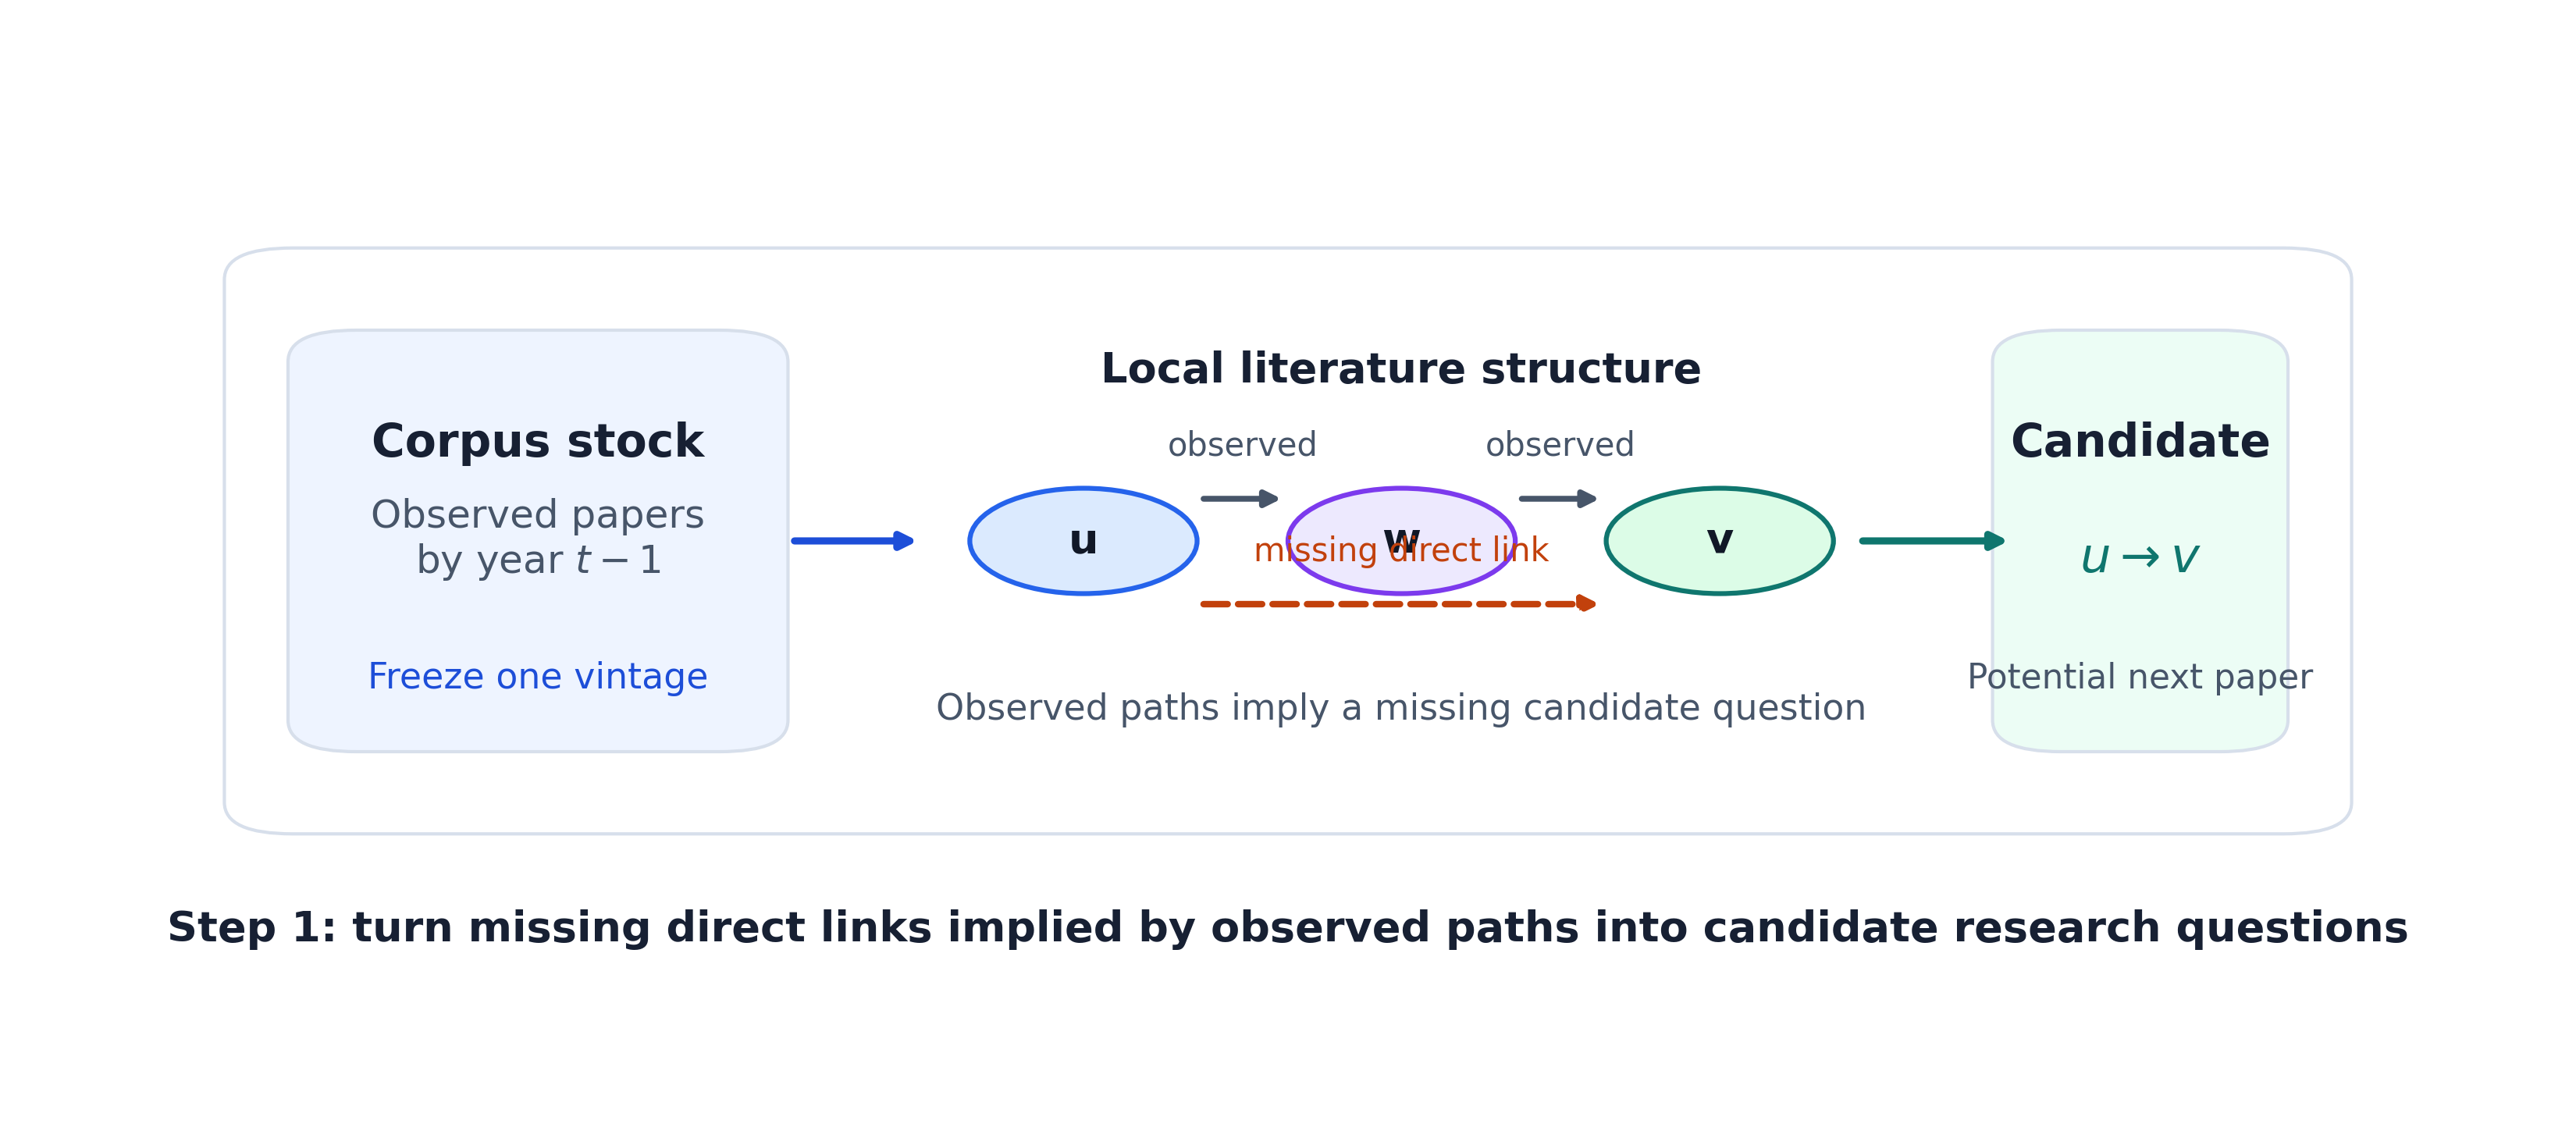
\includegraphics[width=0.90\linewidth]{method_build_step1_candidates.png}
  \caption{Observed local paths can nominate a missing directed link as a candidate next research question.}
\end{figure}

\paragraph{Prospective test.}
Evaluation is prospective. For each cutoff year \(t\), I freeze the graph using only papers observed through \(t-1\), rank missing links, and test whether those links first appear over horizons \(h \in \{3,5,10,15\}\). Those horizons are chosen to span short-run topic scouting, ordinary publication lags, and slower diffusion within economics. I report Recall@100 and mean reciprocal rank. Recall@100 asks what share of future realized links appear inside a shortlist of only 100 candidates; the top-100 threshold is deliberate because the paper is about screening under scarce reading time, not full-universe classification. MRR rewards placing realized links near the top of that shortlist rather than barely inside it. The main benchmark is preferential attachment, defined here as source out-degree times target in-degree. In plain terms, it is a rich-get-richer rule: already central concepts attract more future links even without deeper structural signal.

\paragraph{Results.}
In the pooled rolling benchmark, preferential attachment still outperforms the transparent main model at the strict top-100 shortlist margin. In concrete terms, a 100-paper reading list built from preferential attachment retrieves roughly 2.6, 3.3, 7.0, and 10.0 more realized directed links than the graph score at \(h=3,5,10,15\). That strict-shortlist result is not the whole story. Once the reading budget widens beyond the top 100, the graph-based rule becomes more competitive, and the newer heterogeneity results suggest that pooled averages hide meaningful variation: adjacent journals and design-based causal slices are more favorable terrain for the structural score than the most central core and panel- or time-series-heavy slices.

\begin{figure}[h]
  \centering
  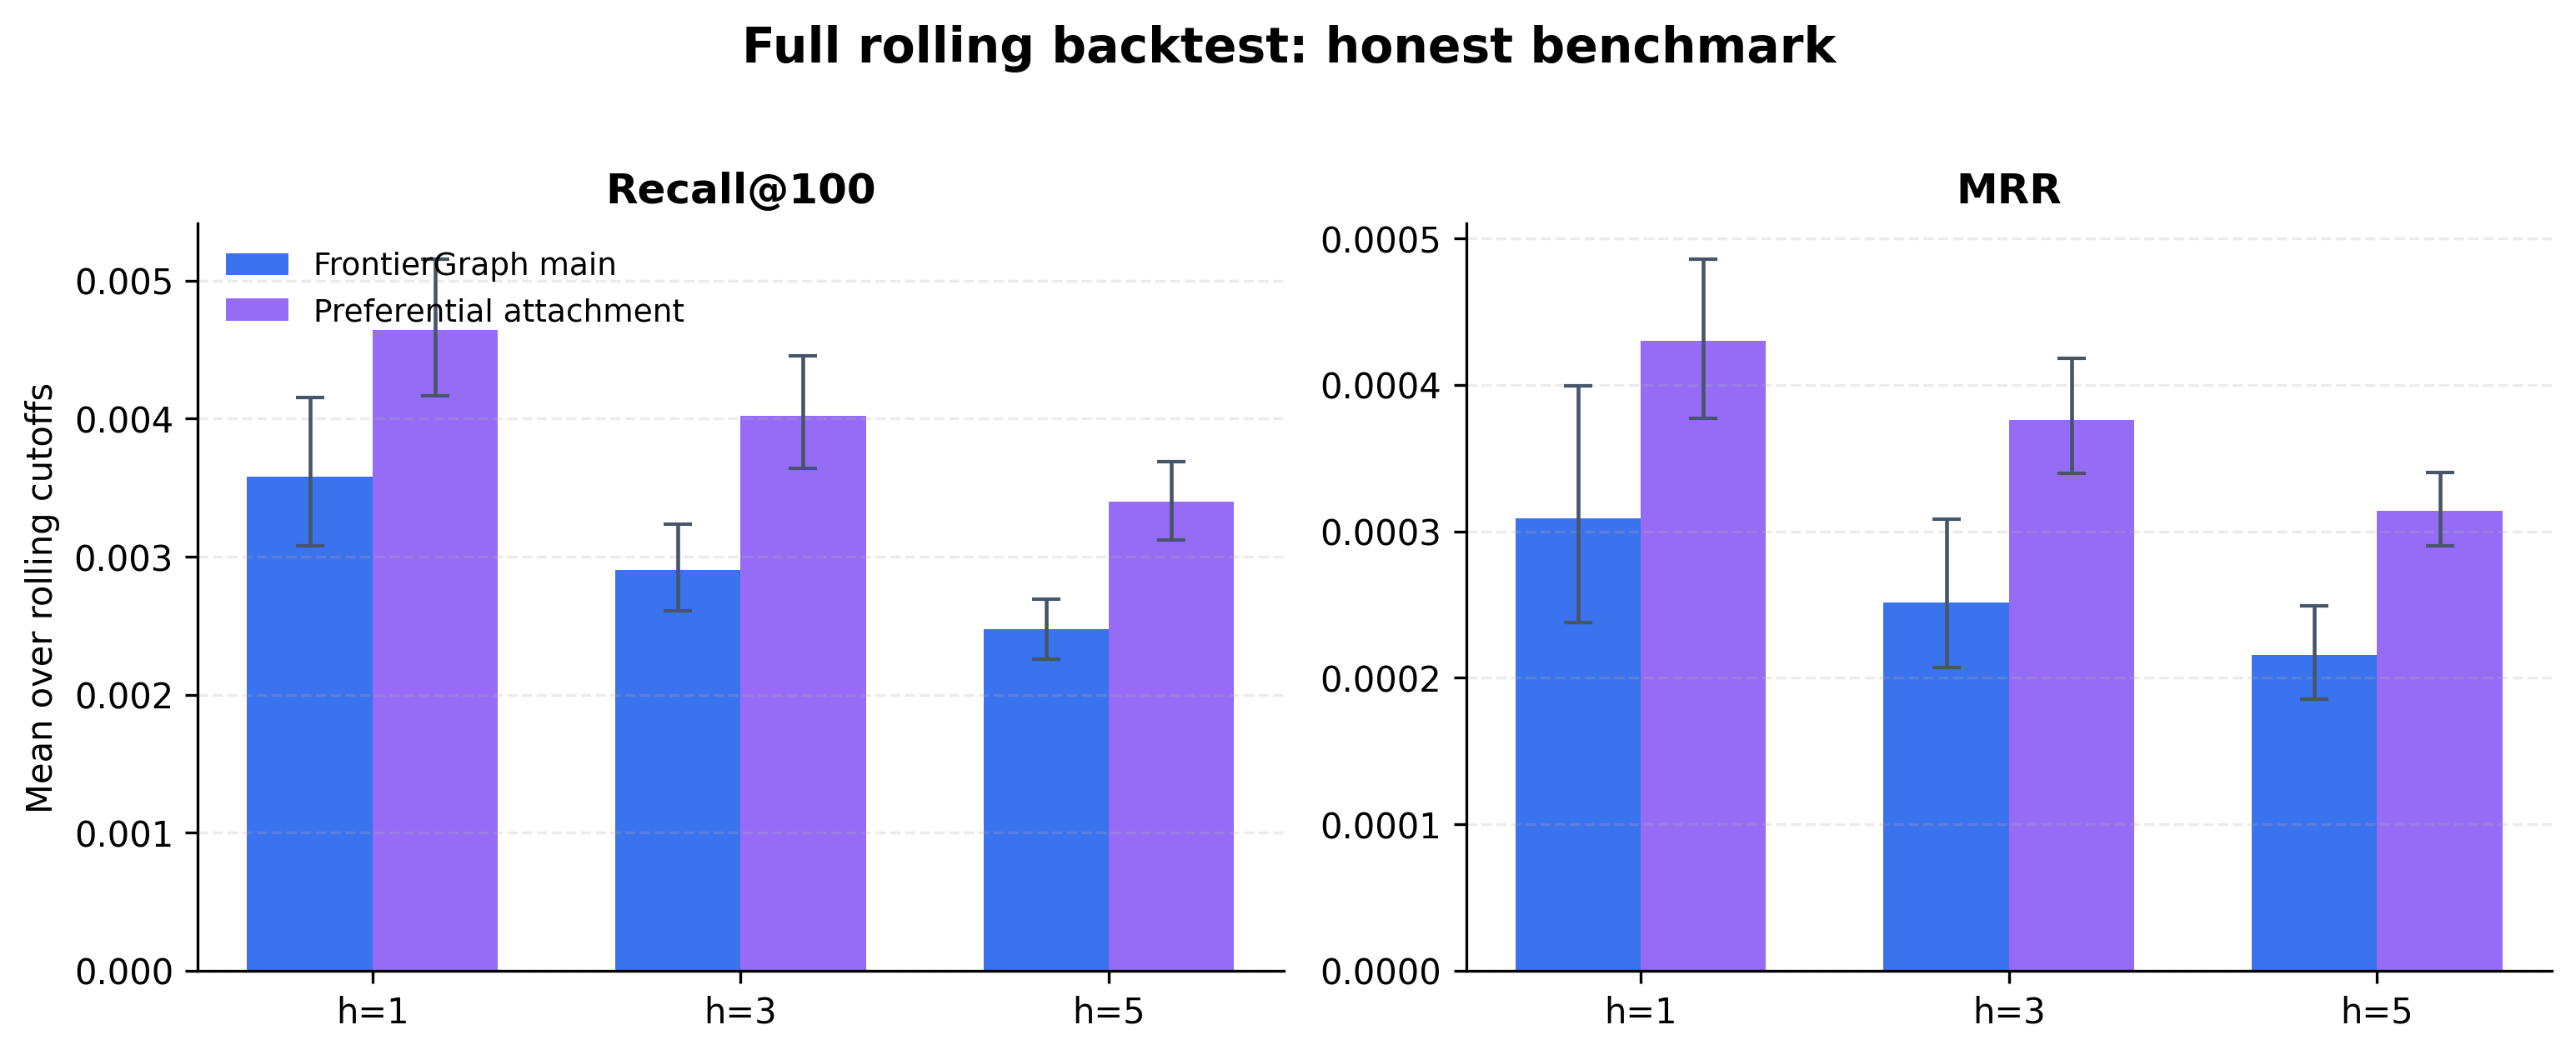
\includegraphics[width=0.90\linewidth]{mainline_full_rolling_vs_pref.png}
  \caption{In the full rolling benchmark, preferential attachment remains stronger than the main transparent model across all tested horizons.}
\end{figure}

\paragraph{Interpretation.}
That is still an informative result for research allocation. The transparent model is not simply a weaker copy of popularity: it is designed to surface questions with stronger local path support and larger direct gaps, even when those questions sit away from the most connected nodes. The substantive distinction I care about is between \emph{gap} questions, which already have nearby support but remain directly underworked, and \emph{boundary} questions, which bridge areas with little or no direct connection.

\begin{figure}[h]
  \centering
  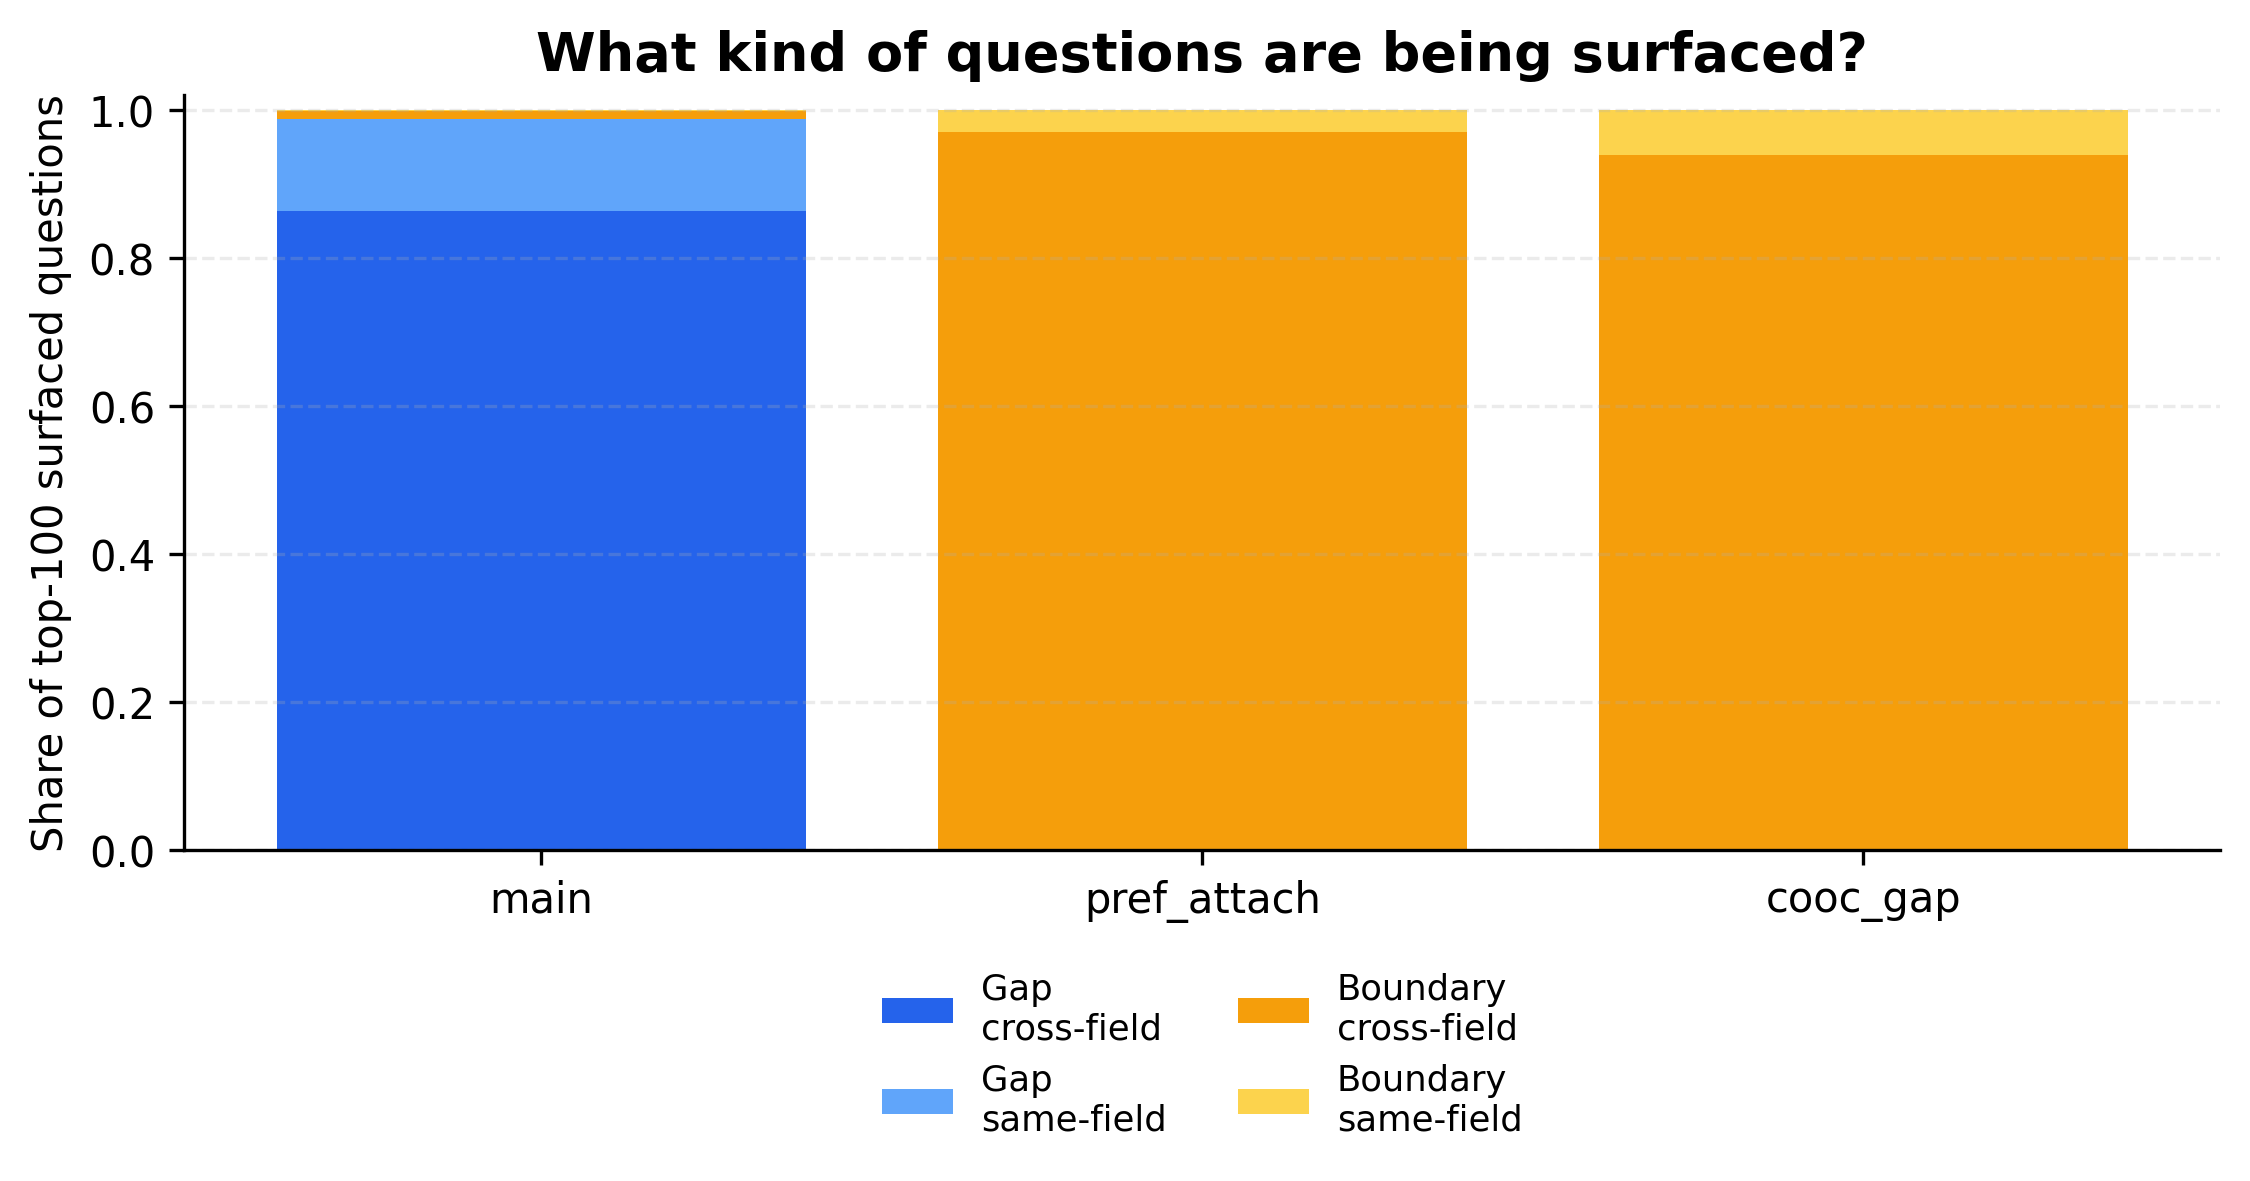
\includegraphics[width=0.78\linewidth]{gap_boundary_mainline.png}
  \caption{Gap and boundary questions are the two substantive types the paper aims to separate within the hybrid claim graph.}
\end{figure}

\paragraph{Path evolution.}
A second result changes how to read the missing-link object itself. A path-evolution audit suggests that the literature often deepens existing direct claims by adding mediator structure more often than it closes a missing direct link already implied by local paths. So the graph is useful not only for surfacing local gaps, but also for showing when a topic may be more likely to evolve through mechanism-building than through direct closure.

\paragraph{Illustrative current questions.}
Current high-ranking outputs from the public layer make the object more concrete. Public debt \(\rightarrow\) CO\(_2\) emissions remains one of the clearest examples: it is supported by 23 nearby paths through concepts such as economic growth, financial development, and renewable energy consumption, and it asks whether debt overhang or fiscal stress spill into environmental outcomes. Monetary policy \(\rightarrow\) energy consumption is another: it is supported by 23 nearby paths and treats energy demand as a neglected transmission channel rather than a purely climate-side outcome. These are illustrative current outputs rather than historical validation evidence, but they show how the ranking combines missing direct links with interpretable local support.

\paragraph{Limits and next steps.}
Several limitations matter for interpretation. A future realized link is not the same thing as causal truth, substantive importance, or policy relevance. Direction in the graph records ordered claim relations, not guaranteed causal identification, and the current score still treats the existence of an edge more seriously than the strength or credibility of the underlying evidence. Even with those qualifications, the contribution is concrete. The paper formalizes candidate next questions as missing links in a hybrid claim graph, evaluates them with leakage-controlled vintage backtests, and turns research allocation in economics into a transparent, prospectively testable empirical object.

\paragraph{Selected references.}
\begin{small}
Bloom, Nicholas, Charles I. Jones, John Van Reenen, and Michael Webb. 2020. ``Are Ideas Getting Harder to Find?'' \textit{American Economic Review} 110(4): 1104--1144.\\
Garg, Prashant, and Thiemo Fetzer. 2025. ``Causal Claims in Economics.'' arXiv:2501.06873. \url{https://arxiv.org/abs/2501.06873}.\\
Zhang, Yue, Xingyu Fan, Hong Wang, Muhan Zhang, and Jie Tang. 2025. ``Exploring the role of large language models in the scientific method: from hypothesis to discovery.'' \textit{npj Artificial Intelligence} 1:14.
\end{small}

\end{document}
